\documentclass{article}
\usepackage[margin=1in]{geometry}
\usepackage{../common}
\usepackage{../pagesetup}

\usetikzlibrary{decorations.pathreplacing}
\usepackage{hyperref}
\usepackage{tikz}
\usetikzlibrary{bayesnet}

\definecolor{ffqqqq}{rgb}{1.,0.,0.}
\definecolor{ududff}{rgb}{0.30196078431372547,0.30196078431372547,1.}
\definecolor{cqcqcq}{rgb}{0.7529411764705882,0.7529411764705882,0.7529411764705882}


\begin{document}

\lecture{11}{October 11}{Sasha Rush}{Jiaoyang Huang}{Belief propagation}

We've seen undirected graph model:
\begin{center}
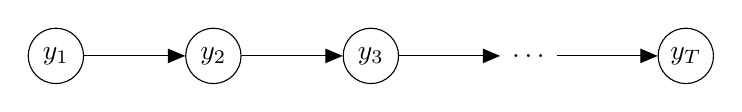
\begin{tikzpicture}
  %Define nodes
  \node[latent]                               (y_1) {$y_1$};
  \node[latent, xshift =2cm]  (y_2) {$y_2$};
  \node[latent, xshift=4cm]    (y_3) {$y_3$};
  \node[latent, draw=none, xshift=6cm] (y_4){$\ldots$};
  \node[latent, xshift=8cm](y_T){$y_T$};

  % Connect the nodes
  \edge {y_1} {y_2} ; %
  \edge{y_2}{y_3}
  \edge{y_3}{y_4}
  \edge{y_4}{y_T}
\end{tikzpicture}
\end{center}
There are many algorithms to do inferences for undirected graph models
\begin{itemize}
\item Forward--backward
\item Sum product algorithm
\item Mean field
\item Belief propagation
\item Gibbs sampling
\item MAP inference.
\end{itemize}

\section{Time series}
We denote the number of classes per node by $V$. The joint probability distributions of times series is given by
\begin{align*}
p(y_{1:T})&=\exp\{\sum_{t}\theta_t^T(y_{t-1},y_t)+\theta_t^{o}(y_t)-A(\theta)\}\\
                &\propto \prod_t\psi_t(y_{t-1},y_t) \psi_t(y_t),
\end{align*}
where $\psi_t(\cdot,\cdot)$ is a binary function, and $\psi_t(\cdot)$ is a unary function. The marginal distribution at $y_s$ is given by
\begin{align*}
p(y_s=v)
&=\sum_{y'_{1:T}\atop y'_s=v}\prod_{t}\psi(y'_{t-1},y_t')\psi(y'_t)/Z(\theta)\\
&=\sum_{y_T'}\psi_T(y_T')\sum_{y_{T-1}'}\psi_{T-1}(y_{T-1}')\psi_T(y_{T-1}', y_{T}')
\cdots \sum_{y_2'}\psi_{2}(y_{2}')\psi_3(y_{2}', y_{3}')\sum_{y_1'}\psi_{1}(y_{1}')\psi_2(y_{1}', y_{2}')
\end{align*}
The sum can be performed in two directions, forwardly from $y_1$, $y_2$ till $y_{s-1}$, and backwardly from $y_T$, $y_{T-1}$ till $y_{s+1}$.
\begin{center}
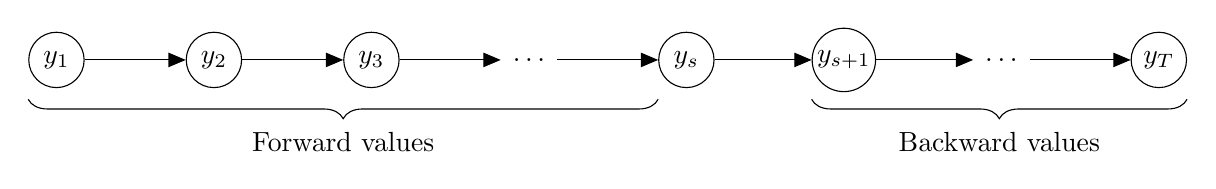
\begin{tikzpicture}[decoration={brace,mirror,amplitude=7}]
  %Define nodes
  \node[latent]                               (y_1) {$y_1$};
  \node[latent, xshift =2cm]  (y_2) {$y_2$};
  \node[latent, xshift=4cm]    (y_3) {$y_3$};
  \node[latent, draw=none, xshift=6cm] (y_4){$\ldots$};
  \node[latent, xshift=8cm](y_s){$y_s$};
  \node[latent, xshift=10cm](y_s+1){$y_{s+1}$};
   \node[latent, draw=none, xshift=12cm] (y_s+2){$\ldots$};
  \node[latent, xshift=14cm](y_T){$y_T$};

  % Connect the nodes
  \edge {y_1} {y_2} ; %
  \edge{y_2}{y_3};
  \edge{y_3}{y_4};
  \edge{y_4}{y_s};
  \edge{y_s}{y_s+1};
  \edge{y_s+1}{y_s+2};
  \edge{y_s+2}{y_T};
  
\draw [decorate] ([yshift=-5mm]y_1.west) --node[below=3mm]{Forward values} ([yshift=-5mm]y_s.west);

\draw [decorate] ([yshift=-5mm]y_s+1.west) --node[below=3mm]{Backward values} ([yshift=-5mm]y_T.east);

\end{tikzpicture}
\end{center}

It takes $O(TV^2)$ steps to compute all margins with dynamic programming, i.e. $p(y_s=v)$ for all $s,v$.

\section{Belief Propagation of Times Series}
We can rewrite the above forward and backward computations in a fancier way. We define forward propagation:
\begin{align*}
\underbrace{{\rm bel}_t^-(y_t)}_{\text{forward belief}}
\propto \psi_t(y_t)
\underbrace{m_{t-1\rightarrow t}^-(y_t)}_{\text{message}},
\end{align*}
where the message is 
\begin{align*}
m_{t-1\rightarrow t}^-(y_t)=\sum_{y_{t-1}}\psi_t(y_{t-1},y_t){\rm bel}_{t-1}^-(y_{t-1}).
\end{align*}
Similarly we define the backward propagation:
\begin{align*}
m_{t+1\rightarrow t}^+(y_t)=\sum_{y_{t+1}}\psi_{t+1}(y_t,y_{t+1})\psi_{t+1}(y_{t+1})m_{t+2\rightarrow t+1}^+(y_{t+1}).
\end{align*}
Then the marginal probability is given by 
\begin{align*}
p(y_t)={\rm bel}_t(y_t)\propto \underbrace{m_{t+1\rightarrow t}^+(y_t)}_{\text{backward}}\underbrace{{\rm bel}_t^{-}(y_t)}_{\text{forward}}.
\end{align*}
To compute all the marginal probability using the above algorithm, it takes $O(TV^2)$ time and $O(TV)$ memory to store all the forward and backward values, i.e. $m_{t+1\rightarrow t}^+(y_t)$ and ${\rm bel}_t^{-}(y_t)$.

\section{Belief Propagation of General Graphs}
We have the belief propagation for time series, it is natural to ask undirected graph model defined by a general graph, 
\begin{align*}
p(y_s=v)=\sum_{y'_{1:T}\atop y_s'=v}\prod_C\psi_C(y_C').
\end{align*}
The above summation might be hard. For example, if $C$ runs through cliques of size $5$, the sum is over $V^5$ terms. Even if we start with a graph with maximum clique size $\leq 2$, the Ising model on $2d$ lattice, we will end up with larger cliques, i.e. cliques of size $3$.

\begin{center}
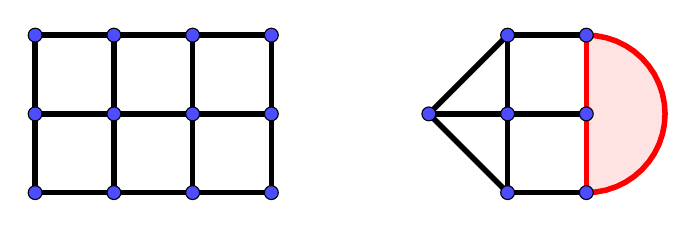
\begin{tikzpicture}[line cap=round,line join=round,>=triangle 45,x=1.0cm,y=1.0cm]
%\draw [color=cqcqcq,, xstep=1.0cm,ystep=1.0cm] (-3.,2.) grid (7.,6.);
%\clip(-3.,2.) rectangle (7.,6.);
\draw [line width=2.pt] (-2.,5.)-- (-1.,5.);
\draw [line width=2.pt] (-1.,5.)-- (0.,5.);
\draw [line width=2.pt] (0.,5.)-- (1.,5.);
\draw [line width=2.pt] (1.,5.)-- (1.,4.);
\draw [line width=2.pt] (1.,4.)-- (0.,4.);
\draw [line width=2.pt] (0.,5.)-- (0.,4.);
\draw [line width=2.pt] (0.,4.)-- (-1.,4.);
\draw [line width=2.pt] (-1.,5.)-- (-1.,4.);
\draw [line width=2.pt] (-2.,5.)-- (-2.,4.);
\draw [line width=2.pt] (-2.,4.)-- (-1.,4.);
\draw [line width=2.pt] (-2.,4.)-- (-2.,3.);
\draw [line width=2.pt] (-2.,3.)-- (-1.,3.);
\draw [line width=2.pt] (-1.,4.)-- (-1.,3.);
\draw [line width=2.pt] (0.,4.)-- (0.,3.);
\draw [line width=2.pt] (1.,4.)-- (1.,3.);
\draw [line width=2.pt] (-1.,3.)-- (0.,3.);
\draw [line width=2.pt] (0.,3.)-- (1.,3.);
\draw [line width=2.pt] (4.,5.)-- (3.,4.);
\draw [line width=2.pt] (3.,4.)-- (4.,4.);
\draw [line width=2.pt] (3.,4.)-- (4.,3.);
\draw [line width=2.pt] (4.,3.)-- (4.,4.);
\draw [line width=2.pt] (4.,5.)-- (4.,4.);
\draw [line width=2.pt] (4.,5.)-- (5.,5.);
\draw [line width=2.pt,color=ffqqqq] (5.,5.)-- (5.,4.);
\draw [line width=2.pt] (5.,4.)-- (4.,4.);
\draw [line width=2.pt,color=ffqqqq] (5.,4.)-- (5.,3.);
\draw [line width=2.pt] (5.,3.)-- (4.,3.);
\draw [shift={(5.,4.)},line width=2.pt,color=ffqqqq,fill=ffqqqq,fill opacity=0.10999999940395355]  plot[domain=-1.5707963267948966:1.5707963267948966,variable=\t]({1.*1.*cos(\t r)+0.*1.*sin(\t r)},{0.*1.*cos(\t r)+1.*1.*sin(\t r)});
\begin{scriptsize}
\draw [fill=ududff] (-2.,5.) circle (2.5pt);
\draw [fill=ududff] (-1.,5.) circle (2.5pt);
\draw [fill=ududff] (0.,5.) circle (2.5pt);
\draw [fill=ududff] (1.,5.) circle (2.5pt);
\draw [fill=ududff] (1.,4.) circle (2.5pt);
\draw [fill=ududff] (0.,4.) circle (2.5pt);
\draw [fill=ududff] (-1.,4.) circle (2.5pt);
\draw [fill=ududff] (-2.,4.) circle (2.5pt);
\draw [fill=ududff] (-2.,3.) circle (2.5pt);
\draw [fill=ududff] (-1.,3.) circle (2.5pt);
\draw [fill=ududff] (0.,3.) circle (2.5pt);
\draw [fill=ududff] (1.,3.) circle (2.5pt);
\draw [fill=ududff] (4.,5.) circle (2.5pt);
\draw [fill=ududff] (3.,4.) circle (2.5pt);
\draw [fill=ududff] (4.,3.) circle (2.5pt);
\draw [fill=ududff] (4.,4.) circle (2.5pt);
\draw [fill=ududff] (5.,5.) circle (2.5pt);
\draw [fill=ududff] (5.,4.) circle (2.5pt);
\draw [fill=ududff] (5.,3.) circle (2.5pt);
\end{scriptsize}
\end{tikzpicture}
\end{center}

The minimum size of max clique induced $-1$ is the \emph{treewidth} of a graph. Calculating the tree width of a graph is $NP$ hard, and can be reduced to $3$-SAT. 


\subsection{Belief Propagation on graphs with treewidth $=1$}
We derive the generalization of forward-backward sum product algorithm on trees.
\begin{center}
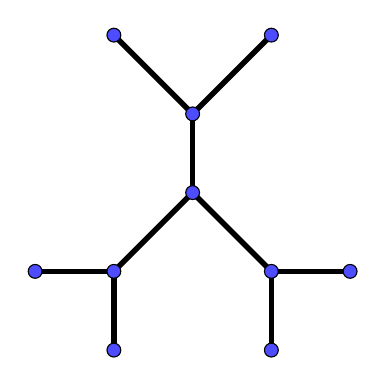
\begin{tikzpicture}[line cap=round,line join=round,>=triangle 45,x=1.0cm,y=1.0cm]
\draw [line width=2.pt] (1.,3.)-- (0.,4.);
\draw [line width=2.pt] (1.,3.)-- (2.,4.);
\draw [line width=2.pt] (1.,3.)-- (1.,2.);
\draw [line width=2.pt] (1.,2.)-- (0.,1.);
\draw [line width=2.pt] (1.,2.)-- (2.,1.);
\draw [line width=2.pt] (2.,1.)-- (2.,0.);
\draw [line width=2.pt] (2.,1.)-- (3.,1.);
\draw [line width=2.pt] (0.,1.)-- (-1.,1.);
\draw [line width=2.pt] (0.,1.)-- (0.,0.);
\begin{scriptsize}
\draw [fill=ududff] (1.,2.) circle (2.5pt);
\draw [fill=ududff] (0.,1.) circle (2.5pt);
\draw [fill=ududff] (2.,1.) circle (2.5pt);
\draw [fill=ududff] (1.,3.) circle (2.5pt);
\draw [fill=ududff] (-1.,1.) circle (2.5pt);
\draw [fill=ududff] (0.,0.) circle (2.5pt);
\draw [fill=ududff] (2.,0.) circle (2.5pt);
\draw [fill=ududff] (3.,1.) circle (2.5pt);
\draw [fill=ududff] (0.,4.) circle (2.5pt);
\draw [fill=ududff] (2.,4.) circle (2.5pt);
\end{scriptsize}
\end{tikzpicture}
\end{center}
For a tree graph, we can pick any vertex as a root, then for any vertex $x_s$ the parent nodes set $pa(x_s)$ and children nodes set $ch(x_s)$ are well defined. The belief propagation consists of two parts: upward pass and downward pass. The upward pass is defined by
\begin{align*}
m_{s\rightarrow t}^-(x_t)&=\sum_{x_s}\psi_{s,t}(x_s,x_t){\rm bel}_s^-(x_s),\\
{\rm bel}_t^-(x_t)&\propto \psi_t(x_t)\prod_{s\in ch(t)}m_{s\rightarrow t}^-(x_t).
\end{align*}
The downward pass is defined by
\begin{align*}
{\rm bel}_s(x_s)&\propto {\rm bel}_s^-(x_s)\prod_{t\in pa(s)}m_{t\rightarrow s}^+(x_s),\\
m_{t\rightarrow s}^+(x_s)&=\sum_{x_t}\psi_{s,t}(x_s,x_t)\psi_t(x_t)\prod_{c\in ch(t),\atop c\neq s}m_{c\rightarrow t}^-(x_t)\prod_{p\in pa(t)}m^+_{p\rightarrow t}(x_t).
\end{align*}
To compute all the marginal probability using the above belief propagation, it takes $O(TV^2)$ time and $O(TV)$ memory.

\section{Some Remarks}
\begin{enumerate}
\item
\end{enumerate}







\end{document}

